\documentclass[10pt,a4paper]{article}
\usepackage[utf8]{inputenc}
\usepackage[T1]{fontenc}
\usepackage[margin=1.6cm]{geometry}
\usepackage{amsmath,amssymb,amsthm}
\usepackage{tikz}
\usepackage{pgfplots}
\pgfplotsset{compat=1.18}
\usepackage{xcolor}
\usepackage{booktabs}
\pagestyle{empty}

\definecolor{keep}{HTML}{378ADD}
\definecolor{disc}{HTML}{E24B4A}
\definecolor{front}{HTML}{1D9E75}
\definecolor{area}{HTML}{C8E6D8}

\newtheorem*{definition}{Definition}

\begin{document}

\begin{center}
{\Large\bfseries A Mathematical Model of AutoResearch}\\[3pt]
{\small Inspired by \texttt{karpathy/autoresearch} --- March 2026}
\end{center}

\vspace{0.4em}

\begin{definition}
An \textbf{AutoResearch process} is a discrete-time stochastic optimization
equivalent to a \textbf{(1+1) Evolution Strategy} with elitist selection:
a single solution is maintained, a single variant is proposed at each step,
and the better of the two survives.
The process is fully determined by \textbf{3 parameters} $(\sigma_0,\;\gamma,\;\mu)$
and operates over a fixed budget of $N$ experiments, each lasting $\tau$ seconds.
\end{definition}

\vspace{0.3em}

\noindent\textbf{1.\; Update rule.}\;
Let $\Theta$ be the space of code configurations and
$f\!:\Theta\!\to\!\mathbb{R}^+$ the objective (\texttt{val\_bpb}, lower is better).
At each step $t$ the agent proposes a variant $\theta'_t$:
%
\begin{equation*}
\theta^*_{t+1} = 
\begin{cases}
\theta'_t & \text{if } f(\theta'_t) < f(\theta^*_t) \quad (\textsc{keep})\\[2pt]
\theta^*_t & \text{otherwise} \quad (\textsc{discard})
\end{cases}
\end{equation*}

\noindent\textbf{2.\; Perturbation model.}\;
The agent's modification is modeled as a stochastic perturbation in metric space:
%
\begin{equation*}
f(\theta'_t) = f(\theta^*_t) + \delta_t\,,
\qquad
\delta_t \sim \mathcal{N}(\mu,\;\sigma_t^2)\,,
\qquad
\sigma_t = \sigma_0 \cdot \gamma^{\,t}
\end{equation*}

\noindent\textbf{3.\; The three parameters.}

\vspace{0.3em}

\begin{center}
\renewcommand{\arraystretch}{1.25}
\begin{tabular}{@{}clll@{}}
\toprule
\textbf{Symbol} & \textbf{Name} & \textbf{Range} & \textbf{Meaning} \\
\midrule
$\sigma_0$ & Initial step size & $\sigma_0 > 0$ & How bold the agent's changes are at the start \\
$\gamma$ & Decay rate & $\gamma \in (0,\,1)$ & How fast exploration narrows (like annealing temperature) \\
$\mu$ & Bias & $\mu \leq 0$ & Agent skill: $\mu\!=\!0$ is random, $\mu\!<\!0$ biases toward improvement \\
\bottomrule
\end{tabular}
\end{center}

\vspace{0.2em}

\noindent The keep probability follows from the perturbation distribution:
$\;\Pr[\textsc{keep}] = \Phi\!\bigl(\!-\mu/\sigma_t\bigr)$,\;
which equals $\frac{1}{2}$ when $\mu\!=\!0$ (random agent) and grows as $|\mu|$ increases (skilled agent).

\vspace{0.5em}

\noindent\textbf{4.\; Frontier and cumulative gain area.}\;
The frontier $F(t) = \min_{s \leq t} f(\theta^*_s)$ is non-increasing by construction.
The \textbf{cumulative gain area} measures total improvement over the baseline $f_0$:
%
\begin{equation*}
\boxed{\;\mathcal{A}_N = \sum_{t=1}^{N}\bigl[f_0 - F(t)\bigr]\;}
\end{equation*}

Maximizing $\mathcal{A}_N$ rewards both \emph{fast convergence} (the frontier drops early) and \emph{final depth}
(the frontier reaches a low value). In the symmetric case ($\mu\!=\!0$):
%
\begin{equation*}
\mathbb{E}[\mathcal{A}_N] \approx \frac{\sigma_0}{\sqrt{2\pi}\,(1-\gamma)}\left[N - \gamma\;\frac{1-\gamma^N}{1-\gamma}\right]
\end{equation*}

\begin{center}
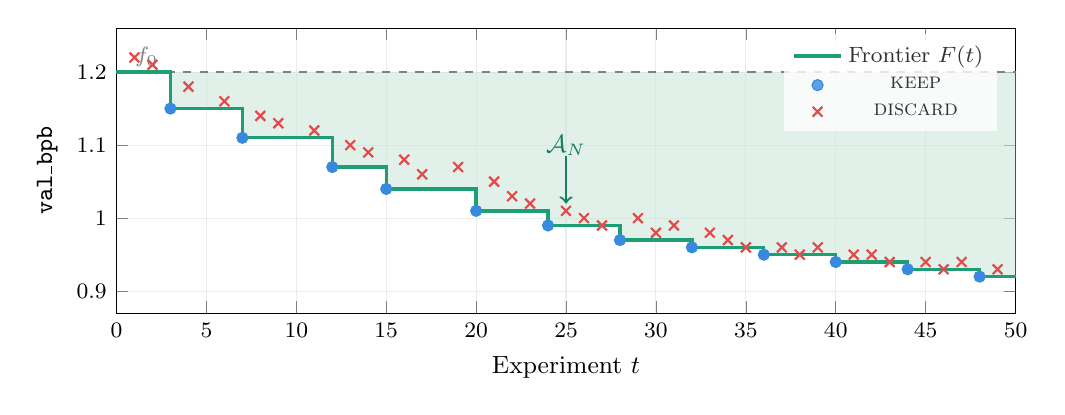
\begin{tikzpicture}
\begin{axis}[
  width=13cm, height=5.2cm,
  xlabel={Experiment $t$},
  ylabel={\texttt{val\_bpb}},
  xmin=0, xmax=50, ymin=0.87, ymax=1.26,
  grid=major, grid style={gray!15},
  tick label style={font=\footnotesize},
  label style={font=\small},
  legend style={at={(0.98,0.98)}, anchor=north east, font=\footnotesize, draw=none, fill=white, fill opacity=0.8},
  clip=false
]

\addplot[fill=area, fill opacity=0.55, draw=none, const plot, forget plot]
  coordinates {
    (0,1.20)(3,1.15)(7,1.11)(12,1.07)(15,1.04)
    (20,1.01)(24,0.99)(28,0.97)(32,0.96)
    (36,0.95)(40,0.94)(44,0.93)(48,0.92)(50,0.92)
  } |- (axis cs:0,1.20) -- cycle;

\addplot[dashed, gray, thick, forget plot]
  coordinates {(0,1.20)(50,1.20)};
\node[font=\footnotesize, gray, anchor=west] at (axis cs:0.5,1.22) {$f_0$};

\addplot[color=front, very thick, const plot]
  coordinates {
    (0,1.20)(3,1.15)(7,1.11)(12,1.07)(15,1.04)
    (20,1.01)(24,0.99)(28,0.97)(32,0.96)
    (36,0.95)(40,0.94)(44,0.93)(48,0.92)(50,0.92)
  };

\addplot[only marks, mark=*, mark size=2pt, color=keep]
  coordinates {
    (3,1.15)(7,1.11)(12,1.07)(15,1.04)
    (20,1.01)(24,0.99)(28,0.97)(32,0.96)
    (36,0.95)(40,0.94)(44,0.93)(48,0.92)
  };

\addplot[only marks, mark=x, mark size=2.5pt, color=disc, thick]
  coordinates {
    (1,1.22)(2,1.21)(4,1.18)(6,1.16)(8,1.14)
    (9,1.13)(11,1.12)(13,1.10)(14,1.09)(16,1.08)
    (17,1.06)(19,1.07)(21,1.05)(22,1.03)(23,1.02)
    (25,1.01)(26,1.00)(27,0.99)(29,1.00)(30,0.98)
    (31,0.99)(33,0.98)(34,0.97)(35,0.96)(37,0.96)
    (38,0.95)(39,0.96)(41,0.95)(42,0.95)(43,0.94)
    (45,0.94)(46,0.93)(47,0.94)(49,0.93)
  };

\node[font=\small\bfseries, color=front!80!black] at (axis cs:25,1.10) {$\mathcal{A}_N$};
\draw[->, thick, front!80!black] (axis cs:25,1.085) -- (axis cs:25,1.02);

\legend{Frontier $F(t)$, \textsc{keep}, \textsc{discard}}

\end{axis}
\end{tikzpicture}
\end{center}

\vspace{-0.5em}

\noindent\textbf{5.\; Trade-offs.}\;
High $\sigma_0$: large jumps, many discards.\;
Low $\sigma_0$: small gains, many keeps.\;
$\gamma \!\to\! 1$: explores longer.\;
Low $\gamma$: converges early, risks local optima.

\smallskip
\noindent\textbf{6.\; Extensions.}\;
\textbf{Multi-agent} ($k$ parallel agents):
$\Pr[\text{at least 1 keep}] = 1-(1-p)^k$.
\;\textbf{Meta-optimization}:
$\texttt{program}^* = \arg\max_{\texttt{prog}}\,\mathbb{E}[\mathcal{A}_N \mid \texttt{prog}]$.

\end{document}